\chapter{Basic Analysis Design}\label{sec:design}

The analysis we will present in  this thesis combines static and dynamic approaches to the QIFC problem. It runs in several stages:

First is a static pre-processing stage. It identifies program parts that are critical to the flow of information and restricts the subsequent analysis to those parts.

Following the pre-processing, a dependency analysis examines possible program executions and evaluates the explicit and implicit information flow along these execution paths. We encode these information flows in propositional formulas and evaluate them using an approximate model counter. The generated boolean predicates can be used to estimate both the channel capacity of the input program as well as the dynamic leakage for a specific execution.

During the evaluation of the channel capacity, the generated boolean predicates might prove to be too complex to be evaluated by a model counter. In this case, our tool will split the program into segments. The segments are analyzed separately and the results are combined for an overall estimation of the program's channel capacity. The analysis of the segments will either be done using the previously generated boolean formulas or by the static QIFC tool Nildumu.

The analysis is integrated into an interpreter that will execute the program for a given input and, additionally to the channel capacity, will give an estimation for the dynamic leakage of the execution.

This chapter will focus on the basic principles of the dependency analysis: The generation of the boolean predicates and the relation between those predicates and the amount of information leaked by the program. For this, we assume that input programs have no loops and no function calls. How these structures can be handled is discussed in section \ref{ch:loops}.

\section{Input Programs}\label{sec:inputLang}

Input programs are written in a variant of the \texttt{while}-language with functions. The language contains the following control structures, using their standard semantics:

\begin{multicols}{2}
    \begin{itemize}
    \setlength\itemsep{0em}
    \item sequential composition
    \item assignments
    \item \texttt{if}-statements
    \item \texttt{while}-statements
    \item \texttt{break}-statements
    \item (recursive) function calls
\end{itemize}
\end{multicols}



The right-hand side of an assignment is an expression that uses the standard arithmetic and bitwise boolean operators. Boolean expressions used in \texttt{while}- and \texttt{if}-statements are defined in the standard way. As already mentioned, we disallow loops and function calls in our input programs for now.

We continue to use the notations introduced in section \ref{p:input} for the input program. Furthermore,  we denote the set of all statements (expressions) that are part of the language as $\stmts$ ($\expr$). Subscripts, such as $\stmts_q$ ($\expr_q)$ indicate the set of statements (expressions) that belong to the program part $q$, where $q$ could be a loop, a function, or the program as a whole.

In our analysis, we work with the input's CFG as well as the PDG, both in SSA form. To further navigate the data structures, we use the following definitions:

\begin{definition}[CFG predecessors and successors]\label{def:succPred}
    The functions will return the set of predecessor and successor blocks respectively for the given basic block.
    \begin{align*}
        pred &: \: \bb_p \to 2^{\bb_p}\\
        succ &: \: \bb_p \to 2^{\bb_p}
    \end{align*}
    We assume for $pred(b)$ that the returned set of predecessors for $b$ is ordered and that the order corresponds to the arguments of any $\phi$-functions that might be present in $b$.
\end{definition}

\begin{definition}
    Let $p$ be a program with statements $\stmts_p$ and basic blocks $\mbb_p$. The function
    \begin{center}
        $BB_p: \: \stmts_p \to \mbb_p$
    \end{center}
    returns for every statement $s \in \stmts_p$ the basic block $b \in \bb_p$ that contains the statement $s$.
\end{definition}

\begin{definition}
    Let $p$ be a program with statements $\stmts_p$ and values \val$_p$. The function
    \begin{center}
        $def: \: $\val$_p \to \stmts_p$
    \end{center}
    returns for every $v \in$ \val$_p$ the statement $s \in \stmts_p$, where the value $v$ is defined. Due to $p$ being in SSA form, this location is unique.
\end{definition}

In our analysis, we view all values as bit vectors. All values are signed integers of a fixed width $w$. We represent the numerical value of an integer as a bit vector using the following map:

\begin{definition}[Bit vector]
    The function
    \begin{center}
        $bv: \:  \mathbb{Z} \to \{0, 1\}^w$
    \end{center}
    maps integers to bit vectors of length $w$, where $bv(n)$ is the two's complement representation of the integer $n$.
    The returned value $bv(n)$ is subject to possible over- or underflows, should the number $n$ not be representable as a $w$-bit two's complement number.
\end{definition}

\paragraph{Execution Value}
We alter the definition of $\llbracket p \rrbracket_h: \{L\} \to \mathcal{L}$ to a function 
\begin{center}
    $\llbracket p \rrbracket_h: \: \val_p \to \{0, 1\}^w \cup \{\bot\}$
\end{center} that takes a program value as an argument and returns the numerical value that was assigned during the execution with input $h$. The numerical value is given as a bit vector of the number's two's complement. If in this execution, the value remains undefined, because the corresponding assignment instruction wasn't executed, the function will return $\bot$. Because the program $p$ does not contain loops or function calls, no assignment can be executed more than once. Thus, $\llbracket p \rrbracket_\cdot(\cdot)$ is well-defined.



\section{Foundations of Dependency Analysis}\label{sec:prop}

The aim of the dependency analysis is to generate a vector of propositional formulas for each program value that we call the \emph{dependency vector}.  This vector contains a formula for each bit of the value, that encodes the state of the bit depending on the bits of the input value. More specifically, the formula contains variables that represent the bits of the input value and if we initialize these variables with the bits of an input, the dependency vector of a value will evaluate to its execution value.

\paragraph{Introductory Example}\label{p:intro}
Before giving a detailed explanation of our analysis, we will demonstrate the basic principles in a short example. The program we want to analyze is shown in figure \ref{fig:introEx}. The program takes an input value, performs two bitwise operations on the value, and then leaks the result. 

\begin{figure}
    \centering
    \begin{minipage}{.7\linewidth}
        \begin{algorithm}[H]
            \hspace*{\algorithmicindent} \textbf{Input} \In $:= (\mIn^2 \mIn^1 \mIn^0)$: int \\
            \hspace*{\algorithmicindent} \textbf{Output} $\mOut_1$: int
            \hspace*{1em}
            \begin{algorithmic}[1]
                \State $\mOut_0 \leftarrow \mIn \; \& \; 110_2 \: \: \: \textcolor{blue}{[H^2 \: H^1 \:0]}$
                \State $\mOut_1 \leftarrow \mOut_0 \; | \; 010_2 \: \: \: \textcolor{blue}{[H^2 \: 1 \: 0]}$
            \end{algorithmic} 
        \end{algorithm}
\end{minipage}
\caption{Introductory example program. Behind each line of code, we have written the propositional vector that represents the assigned value}
\label{fig:introEx}
\end{figure}

Analyzing the program line by line, we can formulate conditions for the assigned values that depend on the values and operations used in the assignment expression:
\begin{itemize}
    \item On line 1, the program assigns to the value $L_0$ the result of a bitwise \texttt{\&}-operation. The right-hand operand is a constant. Because the least significant bit of this constant is \texttt{0}, the least significant bit of $L_0$ must also be \texttt{0}. The two left-hand bits of $L_0$ are identical to the corresponding bits in \In. Thus, we can describe the value $L_0$ by the vector $[H^2 \: H^2 \: 0]$.
    \item On line 2, using the same approach as above, we can ascribe to the value $L_1$ the vector $[H^2 \: 1 \: 0]$
\end{itemize}

The dependency vector $[H^2 \: 1 \: 0]$ which we computed for the output value $\mOut_1$, describes all possible output values of the example program. The vector shows that the last two bit of the output are constant and that the most significant bit is equal to the most significant bit of the input. From this information, we can conclude the following:
\begin{itemize}
    \item The \emph{channel capacity} of the example program is $\log_2(2) = 1$, because the program has only two possible outputs: $\mathtt{110}_2$ iff the most significant bit of \In is \texttt{1} and $\mathtt{010}_2$ iff the most significant bit of \In is \texttt{0}.
    \item Given the value of $\mOut_1$ after an execution, we can infer the value of the most significant bit of $\mIn$. We have no information about the other two bits. For any possible output $l = (l^2 l^1 l^0)$, its indistinguishability set is given by $\mathcal{H}_l := \{ (h^2 h^1 h^0) \in \{0, 1\}^3 \: | \: l^2 = h^2\}$. The \emph{dynamic leakage} of a single execution is $\log_2(2^3) - \log_2(2^2) = 1$.
\end{itemize}

\paragraph{Basic Definitions and Notation}
Propositional formulas are made up of boolean constants \bool \: = $\{ \mttt, \mfff \}$, boolean variables $b_i \in $ \textsc{Var}$_\mbool$ and the standard boolean operators $\{ \lnot, \land, \lor, \implies, \iff \}$. \: \bform{} is the set of all boolean formulas over \textsc{Var}$_\mbool$.

In order to relate bit-vectors and propositional formulas to each other, we use the following definitions:

\begin{definition}[Mapping Bits to Boolean Constants]\label{def:b}
The bijective map $\mathcal{B}: \{0, 1\} \to  \mbform$ maps a bit to a boolean constant.
    \begin{center}
    $\mathcal{B}: \{0, 1\} \to \mbform$
    \begin{align*}
        0 &\mapsto \mfff\\
        1 &\mapsto \mttt
    \end{align*}
    \end{center}
Throughout this thesis, we will apply $\mathcal{B}(\cdot)$ and $\mathcal{B}^{-1}(\cdot)$ implicitly where needed.
\end{definition}

\begin{definition}[Mapping Values to Vectors of Boolean Variables]
    The map
    \begin{center}
        $\var: \: \val_p \to  \mbform^w$
    \end{center}
     assigns a vector of fresh propositional variables to a program value. Each boolean variable is used to represent a bit of the value. A boolean variable is fresh if it is not yet used to represent any other bit. This means that for values $v_0 \neq v_1 \in \val_p$ we have $\var(v_0) \cap \var(v_1) = \emptyset$.
\end{definition}
We will later use the function $\var(\cdot)$ to instantiate propositional variable vectors that represent the input value(s) of the program we are analyzing. The dependency vectors we compute are based on the variable set of these variable vectors. They form the so-called \emph{independent set}:

\begin{definition}[Independent Set]
    Let $\{ \mIn_0, ..., \mIn_m \}$ be the set of input values of \pp. The set of boolean variables
    \begin{center}
        $\var_p := \bigcup\limits_{i \in \{1,..., m\}} \var(\mIn_i)$
    \end{center}
    is called the independent set. The independent set defines the variables that are used in propositional formulas during the analysis.
\end{definition}

\paragraph{Dependency Analysis for Explicit Information Flow}

In the introductory example we introduced the idea of the \emph{dependency vector}: A vector of propositional formulas that represents the state of the value's bits in terms of the bits of the input value. In this section, we will explain how the dependency vector can be computed.

\begin{definition}[Expression Evaluation and Dependency Vectors]\label{def:exprEval}
     The function
    \begin{center}
        $\mathcal{E}: \: \expr \to \mbform^w$
    \end{center}
    evaluates program expressions and computes a vector of propositional formulas that represent the expression result. The computation of $\mathcal{E}(e)$ is shown in figure \ref{fig:expr}.
\end{definition}

\begin{definition}[Dependency Vector]
        The \emph{dependency vector} function maps each value to a vector of propositional formulas. For a value $v$ that is defined in a statement as $v := e$, we define:
    \begin{center}
        $dVec: \: \val_p \to \mbform^w$,\\
        $dVec(v) := \mathcal{E}(e)$
    \end{center}
    The map is well-defined since $p$ is given in SSA-form which means that each value is defined exactly once. We use $dVec(v)^i$ to mean the i-th entry of the vector $dVec(v)$.
    \end{definition}

\begin{figure}
    \begin{subfigure}{1\textwidth}
    \centering
        Let $e := n, \quad n \in \mathbb{Z}$\\
        $\mathcal{E}(e) := \mathcal{B}(bv(n))$
        \caption{Constant Values are represented by dependency vectors that contain boolean constants. The vector entries correspond to the two's complement representation of the constant's numerical value.}
    \end{subfigure}
    \bigskip
    \begin{subfigure}{1\textwidth}
        \centering
        Let $e := \mIn$\\
        $\mathcal{E}(e) := \var(\mIn)$
        \caption{Input parameters are represented by a vector of boolean variables. The variables are part of the independent set $\var_p$ of $p$ and dependency vectors of non-input variables are defined as a function of these variables.}
    \end{subfigure}
    \bigskip
    \begin{subfigure}{1\textwidth}
        \centering
        Let $e := v, \quad v \in \val_p$\\
        $\mathcal{E}(e) := dVec(v)$
        \caption{Variable accesses are evaluated to the dependency vector of the accessed variable.}
    \end{subfigure}
    \bigskip
    \begin{subfigure}{1\textwidth}
    \centering
    Let $e := e_0 \oplus e_1$ or $e := \oplus e_0$
       \caption{Dependency vectors of unary or binary arithmetic expressions and unary or binary bitwise boolean expressions are computed using the combinatorial logic of the two's complement. Even though this logic normally operates on bits (either \texttt{0} or \texttt{1}), we can apply the boolean operations also to propositional formulas, without changing their semantics.}
    \end{subfigure}
    \caption{Definition of $\mathcal{E}(e)$ for different types of expressions $e$}\label{fig:expr}
\end{figure}

To assign each value its dependency vector, we compute $\mathcal{E}(e)$, for the expression $e$ that defines the value in question. For accesses to input variables and constants, the evaluation of $\me{\cdot}$ is straightforward. For other expressions, the evaluation of $\mathcal{E}(e)$ usually depends on the dependency vectors of use-values of $e$. We can guarantee that the needed dependency values have previously been computed, if we evaluate the dependency vectors of program values in the order in which the values are defined in the program.

\section{Measuring Information Leakage with Dependency Vectors}\label{sec:leak}

The entries of a value's dependency vector describe on a bit level, which execution value will be assigned to the value for a certain input value. They take into account all data dependencies in the program. Therefore, we are able to capture all explicit information flows using the dependency vectors.

To demonstrate the connection between a value's dependency vector and its execution value for a particular program run, we evaluate the propositional formulas using the following truth assignment:

\begin{definition}[Evaluation of Dependency Vectors]\label{def:val}
    Every concrete input $h \in \mathcal{H}$ for the input value \In induces a truth assignment: Given the concrete input value $h$ for the input variable $\mIn$, we assign the boolean variables in $\var(\mIn)$ the values of the bits in $h$.
    The evaluation of a propositional formula $f$ with respect to the truth assignment induced by the input $h$ will be denoted by $\mathcal{V}_h (f)$.
\end{definition}

Using the truth assignment induced by a particular input $h \in \mathcal{H}$, the dependency vectors fulfill the following theorem:

\begin{theorem}[Equivalence Theorem]\label{thm:equiv}
    Given an input value $h \in \mathcal{H}$ for the program $p$, let $v$ be an arbitrary value in the program $p$. The relation between the dependency vector and the execution value of $v$ is given by:
    \begin{center}
        $\forall 0 \leq i < w: \mathcal{V}_h(dVec(v)^i) \iff \llbracket p \rrbracket_h (v)^i$
    \end{center}
    At this stage, we have not yet introduced the analysis of programs with diverging control flow. For now, the theorem can only be applied to programs with linear control flow. A proof for the theorem is given in appendix \ref{ch:proofEquiv}.
\end{theorem}

Using theorem \ref{thm:equiv}, we can compute both leakage measures with the following lemmata:

\begin{lemma}[Dynamic Leakage]
    Let $p$ be a program with the concrete value $l$ of the output variable \Out{} being leaked to a public output channel during the execution of $p$ with input $h$.
    The size of $l$'s indistinguishability set $\mathcal{H}_l$ is given by the number of models of the formula:
    \begin{center}
        $F_{dyn} : \bigwedge\limits_{0 \leq i < w} \left( \llbracket p \rrbracket_h(\mOut)^i \iff \mathcal{V}_h(dVec(\mOut))^i \right)$
    \end{center}
\end{lemma}

The formula $F_{dyn}$ contains only the boolean variables from the set $\var_p$. Each model of $F_{dyn}$ thus is a truth assignment $\beta: \var_p \to \mbool$.
If for a truth assignment $\beta$ the formula $F_{dyn}$ is fulfilled, the dependency vector of the output, evaluated with respect to this truth assignment, is equivalent to the bit vector $l$. From theorem\ref{thm:equiv}, it follows that the execution of $p$ with the input $h$ induced by $\beta$ will result in the output $l$.

Assuming a uniform distribution of $\mathcal{H}$, the dynamic leakage of the execution of $p$ with the input $h$ is given by
    \begin{center}
        $L_{dyn}(p, h) = \log_2(|\mathcal{H}|) - \log_2(mc(F_{dyn}))$
    \end{center}

\begin{lemma}[Channel Capacity]
    Let $p$ be a program with an output value \Out. Let $o := [o_0 ... o_w]$ be a vector of boolean variables with $o \cap \var_p = \emptyset$.
    
    The number of distinct outputs of $p$ is given by the projected model count of the formula
    \begin{center}
        $F_{cc} : \bigwedge\limits_{0 \leq i < w} \left( o_i \iff dVec(\mOut)^i \right)$
    \end{center}
    with the variables in $o = [o_0, ..., o_w]$ as the set of priority variables.
    Assuming a uniform distribution of $\mathcal{H}$, the channel capacity is given by
    \begin{center}
        $cc(p) = \log_2(mc_o(F_{cc}))$
    \end{center}
\end{lemma}

\section{Dependency Analysis for Implicit Information Flow}
Implicit information flow occurs when an attacker can draw conclusions about the secret inputs by observing the values of the public outputs and then reconstructing the execution path of a program execution. In this section we will extend the dependency analysis from before to include implicit information flows caused by \texttt{if}-statements. Implicit information flows from more complex control flow structures, such as loops and function calls, are discussed in chapter \ref{ch:loops}. Throughout this section, we use the program shown in figure \ref{fig:doubleIf} as an example to demonstrate the individual steps of the analysis.

\begin{figure}
\centering
\begin{minipage}{.4\linewidth}
    \begin{algorithm}[H]
        \hspace*{\algorithmicindent} \textbf{Input} \In: int \\
        \hspace*{\algorithmicindent} \textbf{Output} \Out: int
        \begin{algorithmic}[1]
            \If{$\mIn < 0$}
                \State $\mOut \leftarrow 0$
            \Else
                \State $\mIn \leftarrow \mIn - 1$
                \If{$\mIn < 0$}
                    \State $\mOut \leftarrow 1$
                \Else
                    \State $\mOut \leftarrow 2$
                \EndIf
            \EndIf
    \end{algorithmic} 
    \end{algorithm}
    \end{minipage}
    \hfill
    \begin{minipage}{.55\textwidth}
        \centering
            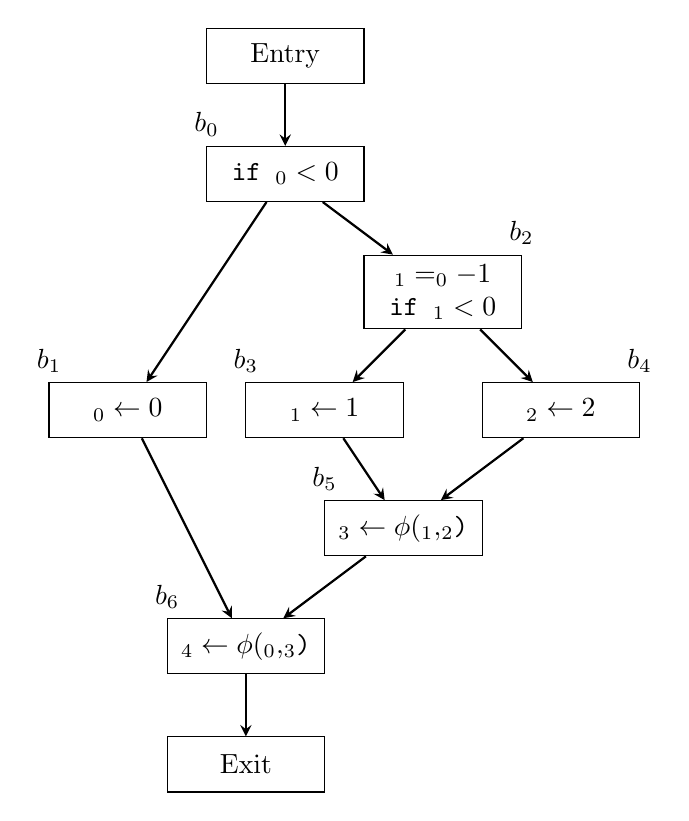
\begin{tikzpicture}
                \tikzstyle{node} = [rectangle, minimum width=2cm, minimum height=.7cm, text centered, draw=black, node distance=1.5cm]
                \tikzstyle{arrow} = [thick,->,>=stealth]
                
                \node (entry) [node] {Entry};
                \node (b1) [node, below of=entry, align=center, label={[xshift=-1cm]$b_0$}] {\texttt{if $\mIn_0 < 0$}};
                \node (b2) [node, below of=b1, xshift=-2cm, yshift=-1.5cm, label={[xshift=-1cm]$b_1$}] {\texttt{$\mOut_0 \leftarrow 0$}};
                
                \node (b3) [node, below of=b1, xshift=+2cm, align = center, label={[xshift=+1cm]$b_2$}] {$\mIn_1 = \mIn_0 - 1$\\\texttt{if $\mIn_1 < 0$}};
                
                \node (b4) [node, below of=b3, xshift=-1.5cm, label={[xshift=-1cm]$b_3$}] {\texttt{$\mOut_1 \leftarrow 1$}};
                \node (b5) [node, below of=b3, xshift=+1.5cm, label={[xshift=+1cm]$b_4$}] {\texttt{$\mOut_2 \leftarrow 2$}};
                \node (b6) [node, below of=b5, xshift=-2cm, label={[xshift=-1cm]$b_5$}] {\texttt{$\mOut_3 \leftarrow
                \phi(\mOut_1, \mOut_2$)}};
                
                \node (b7) [node, below of=b6, xshift=-2cm, label={[xshift=-1cm]$b_6$}] {\texttt{$\mOut_4 \leftarrow
                \phi(\mOut_0, \mOut_3$)}};
                \node (exit) [node, below of=b7] {Exit};

                \draw [arrow] (entry) -- (b1);
                \draw [arrow] (b1) -- (b2);
                \draw [arrow] (b1) -- (b3);
                \draw [arrow] (b2) -- (b7);
                \draw [arrow] (b3) -- (b4);
                \draw [arrow] (b3) -- (b5);
                \draw [arrow] (b4) -- (b6);
                \draw [arrow] (b5) -- (b6);
                \draw [arrow] (b6) -- (b7);
                \draw [arrow] (b7) -- (exit);
            \end{tikzpicture}
    \end{minipage}\hfill
    \caption{Program text and CFG of a short example program. The program returns 0 if $\mIn < 0$, 1 if $\mIn == 0$ and 2 otherwise. The CFG is in SSA-form.}
    \label{fig:doubleIf}
\end{figure}

To include implicit information flow in the analysis, we develop the function $exec: \: \mbb_p \to \mbform$ that assigns each basic block $b$ of a program a propositional formula $exec(b)$ that is fulfilled by the inputs iff the block $b$ is executed. 

In a CFG, the edges represent the jumps between basic blocks. We define the edge condition function $follow: \: \mbb_p \times \mbb_p \to \mbform$ to annotate CFG edges with expressions, that describe when the jump between the two blocks is taken during an execution. The edge annotations are given as propositional formulas, that already take into account the dependency vectors that were computed for the operands. Figure \ref{ex:ec} shows the CFG of the example program \ref{fig:doubleIf} with edges being annotated with their edge conditions.


% might need this later somewhere, not sure
%\begin{definition}[Jump Expression]
 %   For each basic block $b \in \mbb_p$, we define $jump(b)$ as the program expression that decides which successor block of $b$ will be executed.
 %   \begin{center}
 %       $jump: \: \mbb_p \to \mathtt{Expr}$
 %   \end{center}
 %   If $b$ ends in a conditional jump, $jump(b)$ is the expression of the conditional jump instruction.
    
 %   If $b$ ends in an unconditional jump or $b$ is the \texttt{exit} block, we define $b$ as the constant expression \ttt.
%\end{definition}

%\begin{definition}[Edge Condition]
%    Let $CFG(p) = (\mbb_p, E)$ be the CFG of the program $p$.We define
%    \begin{center}
%        $follow: E \to \mbform$\\
%        $(b_0, b_1) \mapsto 
%        \begin{cases}
%            \mathcal{E}(jump(b_0)) & \text{if the execution follows $e$ for $jump(b_0) = \mttt$}\\
%            \lnot \mathcal{E}(jump(b_0)) & \text{if the execution follows $e$ for $jump(b_0) = \mfff$}
%        \end{cases}$
%    \end{center}
%    For every edge $e := (b_0, b_1) \in E$, the propositional formula $follow(e)$ is true iff the control flow during an execution of $p$ jumps from $b_0$ to $b_1$.
%\end{definition}

\begin{figure}
    \centering
                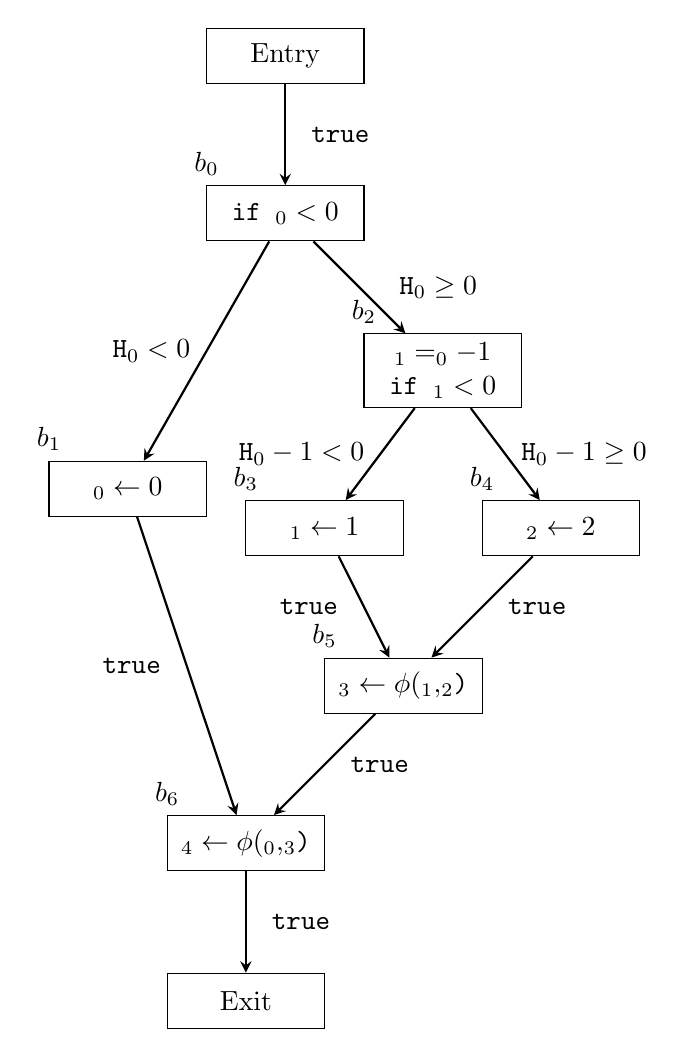
\begin{tikzpicture}
                \tikzstyle{node} = [rectangle, minimum width=2cm, minimum height=.7cm, text centered, draw=black, node distance=2cm]
                \tikzstyle{arrow} = [thick,->,>=stealth]
                
                \node (entry) [node] {Entry};
                \node (b1) [node, below of=entry, align=center, label={[xshift=-1cm]$b_0$}] {\texttt{if $\mIn_0 < 0$}};
                \node (b2) [node, below of=b1, xshift=-2cm, yshift=-1.5cm, label={[xshift=-1cm]$b_1$}] {\texttt{$\mOut_0 \leftarrow 0$}};
                
                \node (b3) [node, below of=b1, xshift=+2cm, align = center, label={[xshift=-1cm]$b_2$}] {$\mIn_1 = \mIn_0 - 1$\\\texttt{if $\mIn_1 < 0$}};
                
                \node (b4) [node, below of=b3, xshift=-1.5cm, label={[xshift=-1cm]$b_3$}] {\texttt{$\mOut_1 \leftarrow 1$}};
                \node (b5) [node, below of=b3, xshift=+1.5cm, label={[xshift=-1cm]$b_4$}] {\texttt{$\mOut_2 \leftarrow 2$}};
                \node (b6) [node, below of=b5, xshift=-2cm, label={[xshift=-1cm]$b_5$}] {\texttt{$\mOut_3 \leftarrow
                \phi(\mOut_1, \mOut_2$)}};
                
                \node (b7) [node, below of=b6, xshift=-2cm, label={[xshift=-1cm]$b_6$}] {\texttt{$\mOut_4 \leftarrow
                \phi(\mOut_0, \mOut_3$)}};
                \node (exit) [node, below of=b7] {Exit};

                \draw [arrow] (entry) -- (b1) node[midway, xshift=.7cm] {\texttt{true}};
                \draw [arrow] (b1) -- (b2) node[midway, xshift=-.7cm] {$\mathtt{H}_0 < 0$};
                \draw [arrow] (b1) -- (b3) node[midway, xshift=1cm] {$\mathtt{H}_0 \geq 0$};
                \draw [arrow] (b2) -- (b7) node[midway, xshift=-.7cm] {\texttt{true}};
                \draw [arrow] (b3) -- (b4) node[midway, xshift=-1cm] {$\mathtt{H}_0 - 1 < 0$};
                \draw [arrow] (b3) -- (b5) node[midway, xshift=1cm] {$\mathtt{H}_0 - 1 \geq 0$};
                \draw [arrow] (b4) -- (b6) node[midway, xshift=-.7cm] {\texttt{true}};
                \draw [arrow] (b5) -- (b6) node[midway, xshift=.7cm] {\texttt{true}};
                \draw [arrow] (b6) -- (b7) node[midway, xshift=.7cm] {\texttt{true}};
                \draw [arrow] (b7) -- (exit) node[midway, xshift=.7cm] {\texttt{true}};
            \end{tikzpicture}
    \caption{CFG from figure \ref{ex:ec} with annotated edges. The annotations represent the formulas $follow(e)$. For easier reading the formulas are given as propositional formulas with linear integer arithmetic instead of bit vector logic.}
    \label{ex:ec}
\end{figure}

\paragraph{Execution Conditions for Basic Blocks}
A basic block $b$ in a program is executed, iff one of its predecessor blocks is executed and the condition for execution to jump from said predecessor to the block $b$ is fulfilled. A special case is a program's entry block, which is executed in every run. This leads to the following definition: 

\begin{definition}[Execution Condition]\label{def:exec}
    For every basic block $b \in \: \mbb_p$, we define its execution condition as:
    \begin{center}
        $exec: \mbb_p \to \mbform$\\
        \begin{align*}
            exec &: BB_p \to \mathcal{F}\\
            exec(b) &:= \begin{cases}
                \mttt &  b = \mathtt{entry}\\
                \bigvee\limits_{p \: \in \: pred(b)} \left( follow(p, b) \land exec(p) \right) & \text{otherwise}\\
        \end{cases}\\
        \end{align*}
    \end{center}
\end{definition}

\begin{lemma}[Basic Block Execution]\label{lemma:exec}
    For every basic block $b \in \: \mbb_p$ and its execution condition $exec(b)$, \\ $\mathcal{V}_h(exec(b)) = \mttt \iff \text{basic block $b$ is executed in a program run with input h}$.
\end{lemma}
The proof for the lemma is given in appendix \ref{ch:proofEquiv} in conjunction with the proof for theorem \ref{thm:equiv}.
\paragraph{Example Computation}
Table \ref{tab:exec} shows the execution conditions of all the basic blocks of example \ref{fig:doubleIf}. We show how these results were computed in detail for blocks $b_3$ and $b_5$:
\begin{itemize}
    \item Basic block $b_3$ has one predecessor $b_2$ with $exec(b_2) = \mIn_0 \geq 0$. The edge $(b_2, b_3)$ represents a conditional jump that is taken iff the condition $follow((b_2, b_3)) := \mIn_0 - 1 < 0$ is fulfilled.
    \begin{align*}
        exec(b_3) &:= follow((b_2, b_3)) &&\land&& exec(b_2) \\
        &= \mIn_0 \geq 0 &&\land&& \mIn_0 - 1 < 0 \\
    \end{align*}
    
    \item Basic block $b_5$ has two predecessors $b_3$ and $b_4$. Their execution conditions are given in table \ref{tab:exec}. Both incoming edges of $b_5$ represent unconditional jumps, thus their edge conditions evaluate to $\mttt$.
    \begin{alignat*}{2}
        exec(b_5) \quad &:= follow((b_3, b_5)) \land exec(b_3) \quad &\lor & \quad follow((b_4, b_5)) \land exec(b_4)\\
        &= \mttt \land (\mIn_0 \geq 0 \land \mIn_0 - 1 < 0) &\lor & \quad \mttt \land (\mIn_0 \geq 0 \land \mIn_0 - 1 \geq 0)\\
        &= \mIn_0 \geq 0 \land (\mIn_0 - 1 < 0 \lor \mIn_0 - 1 \geq 0) \\
        &= \mIn_0 \geq 0
    \end{alignat*}
\end{itemize}

\begin{figure}
    \centering
    \begin{tabular}{ |c|c| } 
        \hline
        $b$ & $exec(b)$ \\
        \hline
        $\mathtt{entry}$ & $\mttt$ \\
        $b_0$ & $\mttt$ \\
        $b_1$ & $\mathtt{H}_0 < 0$ \\
        $b_2$ & $\mathtt{H}_0 \geq 0$ \\
        $b_3$ & $\mathtt{H}_0 \geq 0 \land \mathtt{H}_0 - 1 < 0$ \\
        $b_4$ & $\mathtt{H}_0 \geq 0 \land \mathtt{H}_0 - 1 \geq 0$ \\
        $b_5$ & $\mathtt{H}_0 \geq 0$ \\
        $b_6$ & $\mttt$ \\
        $\mathtt{exit}$ & $\mttt$ \\
        \hline
    \end{tabular}
    \caption{Evaluation of $exec(\cdot)$ for the basic blocks of program \ref{fig:doubleIf}}
    \label{tab:exec}
\end{figure}

\paragraph{Combining Implicit and Explicit Information Flows in $\phi$-functions}
The execution conditions introduced in the previous section can be used to evaluate which basic blocks will be executed depending on the inputs. They contain all control flow dependencies that are present in the program. The formulas describing the implicit flows are integrated into the dependency vectors when a value is assigned the result of a $\phi$-function. Let the value $v_2$ be defined via $v_2 := \phi(v_0, v_1), \: v_0, v_1 \in \val_p$. The assignment expression is part of basic block $b_2$ with predecessors $\{b_0, b_1\}$. The situation is shown in figure \ref{fig:phi}.

To evaluate the $\phi$-expression and compute the dependency vector for value $v_2$, we use the ternary operator $\mathbb{IF}(\cdot, \cdot, \cdot)$:

\begin{definition}[Ternary Operator]
    We define the ternary operator $\mathbb{IF}(\cdot, \cdot, \cdot)$ as:
    \begin{center}
        $\mathbb{IF}: \mbform \times \mbform \times \mbform \to \mbform$\\
        $\mathbb{IF}(c, x, y) := (c \implies x) \land (\lnot c \implies y)$
    \end{center}
    We canonically extend the definition to include propositional vectors:
    \begin{center}
        $\mathbb{IF}: \mbform \times \mbform^k \times \mbform^k \to \mbform^k$\\
        $\mathbb{IF}(c, x, y) := [\mathbb{IF}(c, x^i, y^i)]_{i = 0}^k$
    \end{center}
\end{definition}

The dependency vector of the value $v_2$ can then be computed using the definition of $\mathcal{E}(\cdot)$ for $\phi$-functions given in figure \ref{fig:exprPhi}. The correctness of this definition follows from the following considerations:

If we compute the dependency vector $dVec(v_2) := \mathcal{E}(\phi(v_0, v_1))$ of the value $v_2$, we can assume that the basic block $b_2$ is executed. Otherwise, any assignment to $v_2$ and the information contained in the assignment is irrelevant for the leakage analysis of the execution in question.

If the basic block $b_2$ is executed, at least one of its predecessors $b_0, \: b_1$ must have been executed as well for the execution to reach $b_2$. Furthermore it is impossible for both of $b_2$'s predecessors to have been executed, since so far we only consider loop-free programs, which have no back-edges in their CFG. It follows that the condition $exec(b_0) \veebar exec(b_1)$ must hold for any input value. It is therefore sufficient to check the execution condition of $b_0$ in the definition of $\mathcal{E}(\phi(v_0, v_1))$.

\begin{figure}
\begin{subfigure}{.4\textwidth}
    \centering
    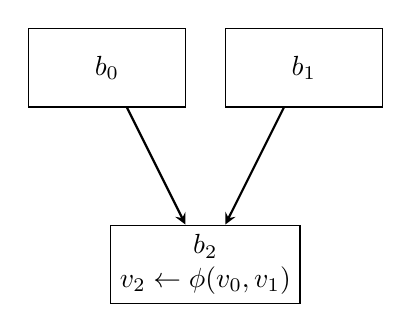
\begin{tikzpicture}
        \tikzstyle{node} = [rectangle, minimum width=2cm, minimum height=1cm, text centered, draw=black, node distance=2.5cm]
        \tikzstyle{arrow} = [thick,->,>=stealth]
                
                \node (b1) [node] {$b_0$};
                \node (b2) [node, right of=b1] {$b_1$};
                \node (b0) [node, below of=b1, xshift=1.25cm, align=center] {$b_2$ \\ $v_2 \leftarrow \phi(v_0, v_1)$};
                
                \draw[arrow] (b1) -- (b0);
                \draw[arrow] (b2) -- (b0);
                
    \end{tikzpicture}
    \caption{Section of a CFG that contains a $\phi$-function.}
    \label{fig:phi}
\end{subfigure}
\hfill
\begin{subfigure}{.5\textwidth}
\vspace{1cm}
    \begin{equation*}
\mathcal{E}(\phi(v_0, v_1)) := \mathbb{IF}(exec(b_0), v_0, v_1)
\end{equation*}
\vspace{1cm}
\caption{Extension of the definition of $\mathcal{E}(\cdot)$ in \ref{fig:expr} for the evaluation of $\phi$-functions.}\label{fig:exprPhi}
\end{subfigure}
\caption{Handling of $\phi$-functions during the dependency analysis}
\end{figure}

\paragraph{Example (cont'd)}
We complete the dependency analysis of the example program \ref{fig:doubleIf} using the algorithm shown in figure \ref{alg:depAna}. The algorithm returns the dependency vector of the leaked value. Figure \ref{fig:exFinished} shows the dependency vectors of all program values. In SSA-form, $\mOut_4$ is the value that corresponds to the program's output. The algorithm returns:
\begin{align*}
    dVec(\mOut_4) &= \mathbb{IF}(\mIn_0 < 0, dVec(\mOut_0), dVec(\mOut_3)) \\
    &= \mathbb{IF}(\mIn_0 < 0, 0, \mathbb{IF}(\mIn_0 \geq 0 \land (\mIn_0 - 1) < 0, dVec(\mOut_1), dVec(\mOut_2))) \\
    &= \mathbb{IF}(\mIn_0 < 0, 0, \mathbb{IF}(\mIn_0 \geq 0 \land (\mIn_0 - 1) < 0, 1, 2))
\end{align*}

\begin{figure}
    \centering
    \begin{algorithm}[H]
        \hspace*{\algorithmicindent} \textbf{Input} $CFG(p) = (\mbb_p, \: E):$ CFG of input program $p$ in SSA form.\\ 
        \hspace*{\algorithmicindent} \textbf{Output} $leaked: \mbform^w$\\
        \begin{algorithmic}[1]
            \State $blocks: (\mbb_p \to \mbform)$
            \State $dVec: (\val_p \to \mbform^w)$
            
            \For{$b \in \mbb_p$ in topological order}
                \State $blocks(b) \leftarrow exec(b)$
                \For{$v := e \in Statements(b)$}
                    \State $dVec(v) \leftarrow \mathcal{E}(e)$
                \EndFor
            \EndFor
            \State $leaked \leftarrow dVec(\mOut)$
    \end{algorithmic} 
    \caption{Dependency Analysis}
\end{algorithm}
    \caption{Algorithm for the dependency analysis of call-free, loop-free programs}
    \label{alg:depAna}
\end{figure}


\begin{figure}
    \centering
    \begin{tikzpicture}
                \tikzstyle{node} = [rectangle, minimum width=2cm, minimum height=.7cm, text centered, draw=black, node distance=3cm]
                \tikzstyle{arrow} = [thick,->,>=stealth]
                
                \node (entry) [node] {Entry};
                \node (b1) [node, below of=entry, align=center, label={[xshift=-1cm]$b_0$}] {\texttt{if $\mIn_0 < 0$}};
                \node (b2) [node, below of=b1, xshift=-2cm, yshift=-1.5cm, label={[xshift=-1cm]$b_1$}] {\texttt{$\mOut_0 \leftarrow 0 \quad \color{blue}{dVec(\mOut_0) = 0}$}};
                
                \node (b3) [node, below of=b1, xshift=+5cm, align = center, label={[xshift=+1cm]$b_2$}] {$\mIn_1 = \mIn_0 - 1 \quad \color{blue}{dVec(\mIn_1) = H_0 - 1}$\\\texttt{if $\mIn_1 < 0$}};
                
                \node (b4) [node, below of=b3, xshift=-2.5cm, label={[xshift=-1cm]$b_3$}] {\texttt{$\mOut_1 \leftarrow 1 \quad \color{blue}{dVec(\mOut_1) = 1}$}};
                \node (b5) [node, below of=b3, xshift=+2.5cm, label={[xshift=+1cm]$b_4$}] {\texttt{$\mOut_2 \leftarrow 2 \quad \color{blue}{dVec(\mOut_2) = 2}$}};
                \node (b6) [node, below of=b5, xshift=-2.5cm, label={[xshift=-1cm]$b_5$}, align=center] {$\mOut_3 \leftarrow
                \phi(\mOut_1, \mOut_2)$\\$ \color{blue}{dVec(\mOut_3) = \mathbb{IF}(\mIn_0 \geq 0 \land (\mIn_0 - 1) < 0, dVec(\mOut_1), dVec(\mOut_2)) }$};
                
                \node (b7) [node, below of=b6, xshift=-5cm, label={[xshift=-1cm]$b_6$}, align=center] {$\mOut_4 \leftarrow
                \phi(\mOut_0, \mOut_3 )$\\$\color{blue}{dVec(\mOut_4) = \mathbb{IF}(\mIn_0 < 0, dVec(\mOut_0), dVec(\mOut_3)) }$};
                \node (exit) [node, below of=b7] {Exit};

                \draw [arrow] (entry) -- (b1);
                \draw [arrow] (b1) -- (b2);
                \draw [arrow] (b1) -- (b3);
                \draw [arrow] (b2) -- (b7);
                \draw [arrow] (b3) -- (b4);
                \draw [arrow] (b3) -- (b5);
                \draw [arrow] (b4) -- (b6);
                \draw [arrow] (b5) -- (b6);
                \draw [arrow] (b6) -- (b7);
                \draw [arrow] (b7) -- (exit);
            \end{tikzpicture}
    \caption{CFG of program \ref{fig:doubleIf} annotated with the dependency vectors of each program value}
    \label{fig:exFinished}
\end{figure}
